\chapter{La gestion des points}

\section{La capture de points}
\subsection{Les \textit{providers}}
\subsection{Le GPS}
\subsection{Le LocationManager}

\section{Projection d'un point}
Comme on a pu le voir dans la partie précédente, la capture de points n'est pas très précise. En effet, pour deux trajets réalisés sur le même parcours, on peut avoir des points situés à des endroits différents et pris à des dates différentes. La figure \ref{Représentation des trajets} représente bien cet écart de prise. Afin de pouvoir comparer deux trajets, nous devons projeter les points (ici le point $A$) du trajet réalisé ($t_2$) sur le trajet de référence ($t_1$). Pour cela nous devons calculer les coordonnées du point $H$ puis le rapport entre $[BH]$ et $[CH]$ afin d'estimer le temps établi pour atteindre le point $A$ sur le trajet $t_1$. Nous pourrons ainsi comparer les temps établis pour atteindre les points $A$ sur $t_2$ et $H$ sur $t_1$.

\begin{img}  
	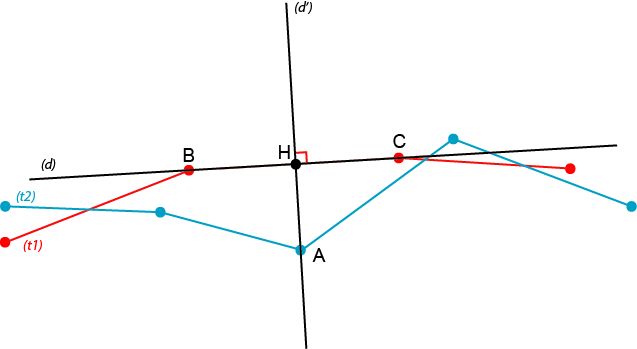
\includegraphics[scale=1]{img/Trajet.png}
	\caption{Représentation des trajets}
	\label{Représentation des trajets}
\end{img}

\subsection{Calcul des coordonnées de H}
On pose trois points $ A(x_a,y_a) $, $ B(x_b,y_b) $ et $ C(x_c,y_c) $ et nous cherchons à calculer les coordonnées de $ H(x_h,y_h) $ (Figure \ref{Représentation des trajets}).
Pour ce faire, nous devons commencer par calculer l'équation de la droite $ d $ passant par les points $B$ et $C$.
On pose donc : 
\[
 d(x) = mx + n
\]
On cherche à déterminer le coefficient directeur de la droite ($m$). Comme $B \in d$ et $C \in d$, on a :
\[
   m =  \frac{x_b-x_c}{y_b-y_c}
\]
Comme le point $B \in (d)$, il résout l'équation :
\[
   y_b = mx_b + n \\
   \Leftrightarrow n = y_b - mx_b
\]
On cherche maintenant à déterminer l'équation de la droite $ d' $ passant par $ A $ tel que $ (d)\bot (d') $. On pose alors, 
 \[
 d'(x) = m'x + n'
\]
Comme $d$ et $d'$ sont orthogonales le produit de leur coefficient directeur est égal à 1, donc:
%\begin{align}
%	mm' = 1 &\Leftrightarrow m' = \frac{1}{m} \\
%        	&\Leftrightarrow (a+b)(a^2+2ab+b^2) \\
%        	&\Leftrightarrow a^3+3a^2b+3ab^2+b^3
%\end{align}
\[
	mm' = 1 \Leftrightarrow m' = -\frac{1}{m}	
\]
d'où
\[
	d'(x) = -\frac{1}{m}x+n'
\]
et comme $ A \in d' $, on a:
\[
	y_a = -\frac{1}{m}x_a + n' \Leftrightarrow n' = y_a + \frac{1}{m}x_a
\]
Comme $ H \in d$ et $H \in d'$, il résout le système suivant :
\begin{align}
    &\begin{cases}
   		 & y_h = -\dfrac{1}{m}x_h + n'\\
   		 & y_h = mx_h + n
    \end{cases} \\
    \Leftrightarrow
    &\begin{cases}
   		& x_h = -my_h + mn'\\
    	& y_h = mx_h + n
    \end{cases} \\
     \Leftrightarrow
    &\begin{cases}
   		& x_h = -my_h + mn'\\
    	& y_h = -y_hm^2 + m^2n' + n
    \end{cases}
\end{align}
\subsection{Interpolation temporelle}

\section{Détermination d'un segment}
\subsection{Les problèmes rencontrés}
\subsection{L'algorithme}